\section{Secure Synthesis}
%Clearly, neither XOR locking or \cite{}'s scheme 

In this section, we first formally capture the intuitive notion of security that a locked netlist must reveal no information about the IP holder's common key. 
%what it means for a locking scheme to be secure . 
We then describe a candidate locking procedure that is secure in this sense. 
%Our candidate procedure involves first representing the Boolean function of a given design in a canonical (yet practically efficient) way. The algorithm then performs locking on the resulting canonical representation.

%describe a candidate construction for a locking scheme that is secure in this sense. 
%We propose a notion of security for a locking procedure, that we argue every locking procedure must satisfy before the procedure can be considered secure. We also propose . 

Before we go any further, we stress that our notion of security --- while enough to protect against our attack --- does not rule out other, more sophisticated attacks; for instance attacks where the fab leverages prior information it has on the design to be fabricated; to deduce the right holder's common key. Towards  the end of this section, we discuss stronger notions of security that protect against this kind of attack, and briefly outline to their potential overheads.

\subsection{Preliminaries}
A traditional synthesis procedure takes as input a description of some desired circuit behaviour and outputs an implementation of the design in terms of logic gates. Unlike previous work \cite{}, we do not treat locking as separate from synthesis; rather we view them as one integrated procedure. Therefore, we extend the definition of a synthesis procedure by allowing to receive along with the behavioral description of a circuit; a bitstring representing a key (which we assume the designer have selected uniformly at random from some key space, of size $2^k$, for integer security parameter $k$), and refer to the new procedure as a \emph{locking synthesis procedure}. Rather than outputting a design implementing the circuit behaviour provided as input, a locking synthesis procedure outputs an ``augmented" design, one that satisfies certain correctness criteria. For simplicity, we assume all RTL descriptions are of single-output circuits which consist of combinational logic only, but we note that all definitions and results are easily extend-able to the multiple-output case as well as sequential logic.

\begin{definition}
A \emph{locking synthesis procedure} takes as input a register-transfer level (RTL) description of a circuit, $f$ (which we model simply as text), and a bitstring $k^{*} \in \{0,1\}^{m}$ of length $m$. We denote by $n$ be the number of circuit inputs in the RTL description $f$. For each $(f,k^*)$-pair, the procedure outputs a circuit $c$ with two sets $x$ and $k$ of $n$ and $m$ inputs respectively. The circuit $c$  satisfies the following correctness criteria (we use $f: X \rightarrow Y$ and $c: X \times K \rightarrow Y$ where $K = \{0,1\}^{m}$, $X = \{0,1\}^{n}$ and $Y = \{0,1\}$ to denote the Boolean functions of $f$ and $c$ respectively):
$$ c(x,k^{*}) = f(x) \, \, \forall x \in X, $$
and 
$$ \exists  x \in X \,\, s.t. \,\, c(x,k) \neq c(x,k^{*}) \, \, \forall k \in K.$$ 
\end{definition}
%For any $x \in X$, the function outputs $y \in Y$ and we say $y = f(x)$.

%To obfuscate the implementation, the defender introduces $m$ key bits, and selects a key $k^{*} \in \{0,1\}^{m}$ uniformly at random. 

%The function that the defender implements (which the attacker sees) is 
%$c: X \times K \rightarrow Y$ where $K = \{0,1\}^{m}$. 
%For any $x \in X$ and $k \in K$, the function outputs $y \in Y$ and we say $y = c(x,k)$.

%The implementation must satisfy the following:
These requirements guarantee that: (1) when the defender applies the correct key, $k^{*}$,
$c$ provides correct outputs for all inputs; (2) when the attacker applies an incorrect, the resulting circuit differs from the correct one for at least one input.

We further extend our definition by allowing a synthesis procedure to be randomized; that is, provided the same circuit description and key as input, two separate executions of the synthesis procedure can result in different outputs (however both must still satisfy the correctness criteria mentioned above).

\subsection{A Notion of Security for Logic Locking}
 Based on the previous definition for a locking synthesis procedure, we now describe our notion of security. The notion is very simple: for every behavioural description, and every key combination (including the correct key), we require that there be a (necessarily distinct) behavioral description, that when locked using the key combination, produces the same locked netlist that the fab observes. 
 
 %We therefore propose that, unless the procedure guarantees \emph{by construction}, and \emph{for every circuit}, that each key is equally likely regardless of the procedure's output (as ensured by our necessary condition for secure synthesis), such a locking procedure should \emph{not} be considered secure.

%Following the principles of secure design, we do not assume a synthesis procedure to be secret; rather we base our security on the secrecy of the correct key $k^*$.

%\subsection{A Necessary Condition}

Formally speaking, let $C(f,k)$ be the random variable describing the output of a synthesis procedure when invoked with description $f$ and key $k$ as input. We define the notion of security as follows.
\begin{definition}
A locking synthesis procedure is secure only if the following condition holds for every behavioural description $f$ and key $k$. For every $k'\neq k$ and $c$ in the support of $C(f,k)$, there exists a behavioural description $f'$ such that
%variables $C(f,k)$ and $C(f',k')$ are statistically indistinguishable. We could opt to require the distributions of $C(f,k)$ and $C(f',k')$ to be perfectly indistinguishable instead; i.e., for each $c$ in the support of $C(f,k)$, 
$P[C(f,k)=c]= P[C(f',k')=c]$
%$$ P(K|C)=P(K) $$ 
(the probabilities are taken over the synthesis procedure's coin flips).

\begin{proposition}
If a secure synthesis procedure additionally satisfies the correctness criteria, such $f'$ cannot be functionally equivalent to $f$.
\end{proposition}
\begin{proof}
\end{proof}

To see how a synthesis procedure satisfying this condition is immune to our attack, consider the following scenario. The rights holder locks a behavioural description $f$, using key $k$. The fab receives the locked netlist $c(f,k)$. Assume for now that all behavioural descriptions are equally likely. Since there are exactly $2^k$ behavioural descriptions that the rights holder could have provided as input to the synthesis procedure (each corresponding to one of the $2^k$ key combinations), and all of which are equally likely, an attacker given $c$ has no way of inferring which of the $2^k$ behavioural descriptions is the correct one (the one provided by the designer as input to the synthesis procedure). Since no two of these $2^k$ description are functionally equivalent (see Prposition ??), an attacker's chance of producing a netlist of the same Boolean function as $f$ becomes exactly $1/{2^k}$.

In practice, however, the assumption that all behavioural descriptions are equally likely does not hold. To see this, consider for instance a circuit that is required to produce $0$ identically as output; regardless of the value provided as input. Such functional behaviour is more likely to be specified in a hardware description language as an output port being set to zero; rather than, say, the AND of two intermediate signals that are complements of each other. \footnote{This is just an extreme example; a reader experienced in VLSI design will identify more realistic ones.} Clearly, if the latter behaviour shows up in the list of candidate behavioural descriptions for a given locked netlist, the fab can immediately discard the description as a potential candidate, assuming, sensibly, that the description could not have possibly been provided by the rights holder as input to the synthesis procedure. In such case, the 
the fab has higher than $1/{2^k}$ chance of obtaining the correct behavioural description.

It is possible to define a notion of security (and construct a procedure) that allows us to slightly relax this assumption. The new notion requires that each Boolean function is equally likely, and makes no assumptions about the relative likelihood of behavioural descriptions for each possible function. We define this notion of security next.

%A locking synthesis procedure is secure if for a every behavioural description $f$ and key $k$, the synthesis output $C$ and key $K$ satisfy 
%$$ P(K|C)=P(K) $$
%where the probabilities above are computed assuming each of the $2^{2^n}$ behaviours that can be provided as input to the synthesis procedure --- are equally likely.
\end{definition}

%This condition does not require $f'$ to be ``likely" to be provided by a chip designer as input to the synthesis procedure, which is why we characterize it as only necessary. It suffices, however, to protect against attacks like ours, where the attacker uses information about the publicly available synthesis procedure to desynthesize the netlist; but does not leverage heuristic knowledge of HDL coding practices.

% The next definition justifies requiring the synthesis tool to function as an IO; if we need the procedure to be resilient to attacks where the attacker might leverage domain knowledge of HDL coding practices.

\begin{definition} Let $F_n$ be the set of all Boolean functions $f_n$ of $n$ variables. For Boolean function $f_n$, let $\gamma_{f_n}$ be the set of all behavioural descriptions (of any size) that implement $f_n$. We model a developer of $n$-input circuits as a distribution ensemble $D_n=\{D_{f_n}\}_{f_n\in F_n}$ where distribution $D_{f_n}:\gamma_{f_n}\rightarrow [0,1]$ describes developer $D_n$'s inclination to describe $f_n$ using each element of $\gamma_{f_n}$. For developer $D_n$, let $C_{D_n}$ denote the random variable describing the output of the synthesis procedure (when the function $f_n$ is selected uniformly at random from $F_n$, and a description is sampled according to $D_{f_n}$). A locking synthesis procedure is secure if for every developer $D_n$ it holds that

$$ P(K|C_{D_n})=P(K) $$

where the probabilities above are taken over the coin flips of the procedure and the developer, and $K$ denotes the locking key.
\end{definition}

Here, again, we note that --- if the synthesis procedure as well satisfies the correctness criteria --- the above condition implies that $P(f_n)>0$ for exactly $2^k$ of the elements of $F_n$ (each of the $2^k$ elements is of course equally likely, by assumption).
%require the condition above to hold for every behavioural description whose Boolean function is equivalent to that of $f'$ (and of course, that the Boolean functions of $f'$'s are distinct from $f$). Formally, for every $g\equiv f'$, 
%the distributions of $C(g,k')$ and $C(f,k)$ should be perfectly/statistically indistinguishable.
%$P[C(f,k)=c]\leq P[C(g,k')=c]$. 

%We should note however that by doing so, we automatically obtain an indistinguishability obfuscator (if, post synthesis, we set the key bits to their correct values).

\begin{proposition}
If, post synthesis, we set the key bits to their correct values, a locking synthesis procedure secure according to the definition above functions as an indistinguishability obfuscator.
\end{proposition}

\begin{proof}
An indistinguishability obfuscator is a (possibly randomized) program that transforms a circuit into an equivalent one and additionally has the following property: if $p_1$ and $p_2$ are two functionally equivalent circuits, the distributions of $IO(p_1)$ and $IO(p_2)$ are statistically indistinguishable ($IO(p)$ denotes the output of the indistinguishability obfuscator when invoked on circuit $p$). Suppose a synthesis procedure satisfied the security notion defined above but did not function as an indistinguishability obfuscator in this sense. This implies that there exists a key $k$, two descriptions $d_1$ and $d_2$ of the same Boolean function $f$, and a $c$ in the support of $C(d_1,k)$ such that $P[C(d_1,k)=c]\neq P[C(d_2,k)=c]$. Now consider a developer $D$ that implements $f$ using $d_1$ or $d_2$ with equal probabilities. For this developer, observing that the output of the synthesis procedure is $c$ changes the prior on $d_n$, which violates the requirement that $P(K|C)=P(K)$.
\end{proof}

%\begin{definition}
%If we define a locking synthesis procedure as accepting a \emph{Boolean function} (rather than a behavioural description of a function), and require, further, that the procedure's output is insensitive to the way the input Boolean function is represented (in other words, that the synthesis procedure is an indistinguishability obfuscator), we can then define our notion of security as follows. Simply, for every $(f,k)$ pair and every $k'\neq k$, there exists a Boolean function $f'$ such that $P[C(f,k)=c]=P[C(f',k')=c]$ for every $c$ in the support of $C(f,k)$.
%\end{definition}

% We note, however, that most practical synthesis tools cannot be precisely characterized as accepting Boolean functions; rather, they typically accept an abstract form of desired circuit behaviour (written for example in an HDL). 
 
\begin{definition}[Other candidate notions of security]
Both notions of security defined above make somewhat unrealistic assumptions about the possible designs that might be provided by a rights holder to the synthesis procedure (after all, there is arguably no use for a design house to design a circuit that outputs $0$ identically; but our assumption implies that such functionality is as likely as any other to be supplied to a locking scheme). An intersting question is whether it is possible to design schemes that make no assumptions whatsoever regarding the adversary's prior information about the design (functionality, description, or otherwise).

The answer to this question is yes. It is possible to construct such schemes. We simply treat circuits as messages to be encrypted, and use a semantically secure message encryption scheme to encrypt the designs. The maskset provided to the fab consists of the encrypted design, an implementation of the decryption procedure of the encryption scheme, followed by a universal circuit that executes the design once it is decrypted. The (private) encryption key is held secret by the rights holder (as a common key). When the key is applied to a fabricated chip, the decryption circuit decrypts the hardwired encryption of the design, and provides the resulting ``plaintext" design for the universal circuit to be executed. 
%do this by borrowing tools from the field of cryptography, where it has long been known that it is possible to design 

The benefit of using a semantically secure message encryption schemes is that such schemes ensure (by construction) that a generated ciphertext reveals no information about the plaintext that can \emph{feasibly} be computed. In our case, this ensures that regardless of what prior information the fab has about the design (functionality, or otherwise); gaining access to the locked netlist (which now ontains only an encryption of the design) does not leak any extra information about the design that can be feasibly extracted. The fab thus remains as able to overbuild the chip after it receives the maskset as it was before receiving the mask.

%This seems to be good news; the downside is that 
%Unfortunately, it appears that the only way is to make use of cryptographic promitives ,the overhead of such techniques might be too xxx to enable a practical application.
%The good news in our case is that we can use one-time, which appear to be somewhat easier to implement that a full-fledged . For example, a simple then use a pseudorandom bit generator to expand the key\cite{}. An attacker . There is also the question of whether it might incur less overhead to simple (remember that in the logic locking setting, there is no overhead of key communication, )

%\paragraph{Conclusion}
%To 
%A locking synthesis procedure is secure if the probability of a PPT adversary winning the following game is negligible (in the key length $k$): the adversary knows the details of the locking procedure, and he performs polynomial time computations of his choice. He then provides the the locking oracle with two circuits $c_1$ and $c_2$ of his choice (they only get to do this \emph{one time}). The locking oracle selects one of $c_1$ and $c_2$ uniformly at random, locks the selected circuit using her locking key, and provides a locked circuit to the adversary. The adversary performs polynomial-time computations of his choice and then guesses which of $c_1$ and $c_2$ was selected by the locking oracle. The adversary wins the game is his guess is correct.
\end{definition}

%The above notion of security may be regarded as too strong. First of all, we do not require every aspect of the design to be protected (none of the existing locking scheme live up to this). We only require that recovering the locking key be impossible (and that programming the key register with an incorrect key results in functionality that is controllably different from the correct functionality). Perhaps we could require the two circuits $c_1$ and $c_2$ provided by the adversary to the oracle to be functionally nonequivalent (we discussed yesterday that if the attacker knows the functionality of the design, we consider him to have broken the locking scheme). I'm not sure how this would make constructing a secure procedure easier; but constructing a universal BDD does seem to be easier than constructing a universal circuit. We can also argue that revealing a BDD's structure (sans edge labellings) is acceptable in our setting, and thus we would only need as many key bits as there are nodes in the BDD.

%In any case, the following construction satisfies the above notion of security: the locking procedure first uses any one-time indistinguishable encryption algorithm to encrypt the input behavioural description. The locked circuit then consists of a circuit implementing the corresponding decryption algorithm (whose plaintext inputs are hardwired to the obtained ciphertext), followed by a universal circuit. This construction would probably have too much area, power and delay overhead to be practical in our setting.

%In this section, we argue that XOR locking (Section ??), and to the best of our knowledge, must not be considered secure; as they all fail to satisfy basic requirement of any information hiding scheme with no c. We Following the principles of secure design, we do not assume a synthesis procedure to be secret; rather we base our security on the secrecy of the correct key $k^*$.

%\subsection{A Necessary Condition}
%Intuitively, a synthesis procedure must at a minimum make it ``hard" --- if at all possible --- for a malicious entity at a fab to recover the correct key from an encrypted design. To make an analogy to the traditional setting of encryption, this is similar to say that it must be hard or impossible for an eavesdropper to correctly guess a sender's secret key simply by observing encrypted communication between the sender and a receiver \footnote{the settings are not exactly the same as unlike most settings where encryption is used, here the ``eavesdropper" only gets to read a \emph{single} message; the sender also gets to change the encryption key prior to sending a new communication}. Cryptographic protocols usually ensure this by making key deduction equivalent (or at least as hard as) solving a computational problem known to be xxxx hard. Common examples are integer factoring and the discrete logarithm problems \cite{}. This is know as the computational hardness approach to security \cite{}.

%Another approach, the information theoretic one \cite{} is to xxxx make a plaintext absolutely independent of the ciphertext, \footnote{In cryptography, this is known to be possible to achieve only when the key space is as large as the message space \cite{}. Therfore, information theoretic security, while intuitively preferrable, is usually foregone in xxxx of computational security, which is possible to achieve even given key spaces of limited size (security is parameterized by the key length)}where independence is xxxx in a probabilitstic sense, i.e., if $X$ is a random variable that denotes the plaintext, and $Y$ is the random variable that denotes the ciphertext, then the probability distributions of the two variables must satisfy:

%$$ P(X|Y) = P(X) $$

%In our setting, we seek to protect the locking key; and what the attacker has access to is an encrypted netlist output by a synthesis procedure as defined in Section ??. We there argue that a \emph{necessary} condition of secure synthesis is:

%\begin{proposition}
%A locking synthesis procedure as defined in Section ?? is secure only if for every behavioural description $f$, the synthesis output $C$ and key $K$ satisfy 
%$$ P(K|C)=P(K) $$
%where the probabilities above are computed assuming each of the $2^{2^n}$ behaviours that can be provided as input to the synthesis procedure --- are equally likely, and that for each behaviour, all descriptions are equally likely to be provided as input.
%\end{proposition}

%The condition in Proposition ?? ensures that given the unencrypted netlist, knowledge of the encrypted netlist does not reduce uncertainty about the locking key. %Is this condition sufficient by itself to guarantee impossibility of key recovery? No. As a counter-example, consider a synthesis procedure that produces, for an input behavioral description, a implementation that, for all keys other than the correct one, behaves as specified by the input description, for all inputs save one (a fixed value for all keys). The construction in Figure?? is one example of such implementation The comparator checks wether the input key . Such synthesis procedure is clearly secure according to Condition 1; the input correct key value is not used at all when constructing the encrypted design; therefore the locked design produced is the same for all input keys, i.e., it is independent of the correct key value. Such a locking 
%We therefore introduce another condition for secure synthesis:
%\begin{proposition}
%A synthesis procedure as defined in Section ?? is secure only if 
%\end{proposition}
%Such a condition rules out procedures like the one in Figure ??.
%Note that we assume that for every behaviour, all descriptions are equally likely \footnote{It can be argued that not all descriptions are likely for a given desired behaviour; e.g, if the circuit is required to produce $0$ identically as output, this is more likely to be specified in VHDL as an output port being set to zero; rather than the AND of two intermediate signals that are complements of each other. This is just an extreme example; a reader experienced in VLSI design will identify more realistic ones.}. This is why the condition is necessary.

\subsection{A Candidate Secure Synthesis Procedure}
We now propose a candidate locking procedure that not only meets our necessary condition for secure synthesis, but also allows to easily ensure the correctness criteria of locking synthesis are satisfied. We first provide a brief introduction to a concept in  that is critical to understanding our technique, that is of binary decision diagrams. 
%A reader familiar with binary decision diagrams can skip directly to Section ??.

\subsubsection{Binary Decision Diagrams}
A binary decision diagram (BDD) is a way of representing a Boolean function in terms of a graph that describes the Boolean calculations performed by the function. Given an assignment to the input variables of the function, an evaluator starts at the root of the diagram and proceeds by selecting one of the two children the current node, based on the value of the variable associated with the node. This continues until the evaluator reaches a leaf node, which specifies the value taken by the function at that particular sequence of input values. As an example, a BDD for representing the function $f = a \equiv b$ is shown in Figure ??.

%% This part makes a figure
\begin{figure}[ht]
  \dummyfig{Dummy Figure Label} 
  \caption{A BDD representing the function $f = a \equiv b$. The high and low children of a decision node are discriminated by using a solid (dotted) line to draw the edge leading to the high (low) child.}
  \label{fig:dummy2}
\end{figure}

More formally, a BDD can be defined as a rooted directed acyclic graph with two types of nodes: \emph{decision} and \emph{terminal} nodes. A terminal node can be either a $0$-terminal or a $1$-terminal, and there can be at most two terminal nodes in a BDD. Each decision node, $N$, is labeled with a variable $V_N$ and has two child nodes: a low child and a high child. The edge from $V_N$ to its low (or high) child represents an assignment of $V_N$ to $0$ (respectively $1$). A path from the root node to the $1$-terminal represents a variable assignment for which the Boolean function is true. Similarly, a path to the $0$-terminal represents a variable assignment for which the Boolean function is false. Note that given a BDD representation of a function, we can easily build a Boolean circuit that decides the function, for instance, by replacing each decision node $N$ with a 2-to-1 multiplexer that uses $V_N$ the its select line. This is illustrated in Figure ???.

\begin{figure}[ht]
  \dummyfig{Dummy Figure Label} 
  \caption{A BDD representing the function $f = a \equiv b$. The high and low children of a decision node are discriminated by using a solid (dotted) line to draw the edge leading to the high (low) child.}
  \label{fig:dummy3}
\end{figure}

BDDs as a way of representing Boolean functions are special, in that a BDD is a canonical representation of its corresponding Boolean function:, i.e., if we fix the input variable order, there is only one way to represent a Boolean function using a BDD \cite{}. Moreover, unlike a truth table (another canonical representation), the size of a BDD is not always exponential in the number of input variables. These two facts together form the basis for the data structure use in a wide variety of applications \cite{}. Canonicality, in particular, plays a key role for our construction of a secure synthesis procedure, as will become apparent shortly.
%\footnote{One might wonder why we require the to be probably only; rather than requiring the outputs for both description-key pairs to be identically distributed. We argue that since an encryption key here is used only one time}

%An overview of the various logic locking technique that has been proposed in the literature:
\subsubsection{The Procedure}

We now describe a locking synthesis procedure that meets the necessary condition for security introduced in Section ??. A striking feature of our procedure (or perhaps the necessary condition) is that it enables any transformation to be applied on resulting implementations (provided of course the transformation is functionality-preserving), without compromising security at all. We formalize this in the following lemma.

\begin{lemma}\label{simple}
Let $T$ be a functionality-preserving transformation, and denote by $s \circ t$ the (correct) synthesis locking procedure we obtain by composing $T$ with a locking synthesis procedure $s$. If $s$ satisfies the necessary condition for security of Proposition ??, the so does $s \circ t$. 
\end{lemma}
The proof of the lemma is straightforward.

Our synthesis procedure takes the RTL description provided as input, and uses it to constructs a corresponding Boolean network. The BDD representation of the output variable's Boolean function is then computed (recall that we are assuming an RTL description of a single-output circuit). This BDD is then written in a compact form (), and modified to obtain a ``locked BDD". The locked BDD is then converted to a Boolean circuit, which is finally provided as output of the synthesis procedure. If a designer so wishes, they can then feed this circuit to a logic synthesis tool to further optimize it (or to perform technology mapping and obtain an implementation in terms of logic gates); thanks to Lemma \ref{simple}, they can be sure that these further operations on the circuit will in no way affect the security property.  We next describe each of the xxxx steps in detail, then prove that our procedure satisfies the necessary condition for secure synthesis in Section ??.

%The first step
In a standard BDD representation, every node can be thought of as representing an ``intermediate" Boolean function that defines the behavior of the ``overall" Boolean function for a specific partial variable assignment (the assignment represented by the path from the root to the node in question). Let $N_h$ and $N_l$ be the high and low children, respectively, of decision node $N$, and let $f_{I}$ be the Boolean function represented by node $I$.  We can then write,

\[f_N=V_N f_{N_h}+V_N' f_{N_l}\]

Note that if we switch the polarities of $N_h$ and $N_l$, the function represented by node $N$ becomes:

\[f_N^*=V_N' f_{N_h}+V_N f_{N_l}\]

We convert the standard BDD representation to a ``compact" representation in which a decision node $N$ represents both functions, and we signify this in a graph using ``bubbled" nodes. An incoming edge to a decision node $N$ can either terminate at the ``main" part or the ``bubble" part of $N$, to indicate which of the two functions $f_N$ and $f_N^*$ defines the behavior of the overall function for the corresponding partial variable assignment. An BDD can be converted into this form by simply looking for ``complement" nodes (a pair of nodes labeled with the same variable and that has the same children as each other; with different polarities), and replacing each pair with a single ``bubbled" node, preserving original ROBDD edge connectivity. Note that looking for such nodes is easy (we need to perform $O(N^2)$ comparisons, where $N$ the maximum number of nodes at any level in the BDD). An example is shown in Figure ??. Note that since the conversion procedure operates on BDDs --- a canonical representation --- and is deterministic, the resulting representation of the Boolean function must also be canonical. We call the new compact representation a \emph{bubbled} BDD.

\begin{lemma}

\end{lemma}

\begin{figure}[ht]
  \dummyfig{Dummy Figure Label} 
  \caption{A BDD representing the function $f = a \equiv b$. The high and low children of a decision node are discriminated by using a solid (dotted) line to draw the edge leading to the high (low) child.}
  \label{fig:dummy4}
\end{figure}

\paragraph{Encryption Procedure}  To encrypt the new BDD, we pick $k$ nodes at random and insert a new node for each as a descendant, in the manner shown in Figure ??. Each of the new $k$ nodes is then labeled with the variable corresponding to a distinct key bit. If the value of the corresponding key bit is $1$, the polarity of node $N$'s children with respect to the new key node, is preserved; otherwise, children polarities are flipped (low becomes high and high becomes low). %The resulting BDD is then fed into a synthesis tool (after conversion into a circuit) to obtain the final implementation.

\begin{figure}[ht]
  \dummyfig{Dummy Figure Label} 
  \caption{A BDD representing the function $f = a \equiv b$. The high and low children of a decision node are discriminated by using a solid (dotted) line to draw the edge leading to the high (low) child.}
  \label{fig:dummy5}
\end{figure}

%\begin{figure*}[!htb]
%\centering
%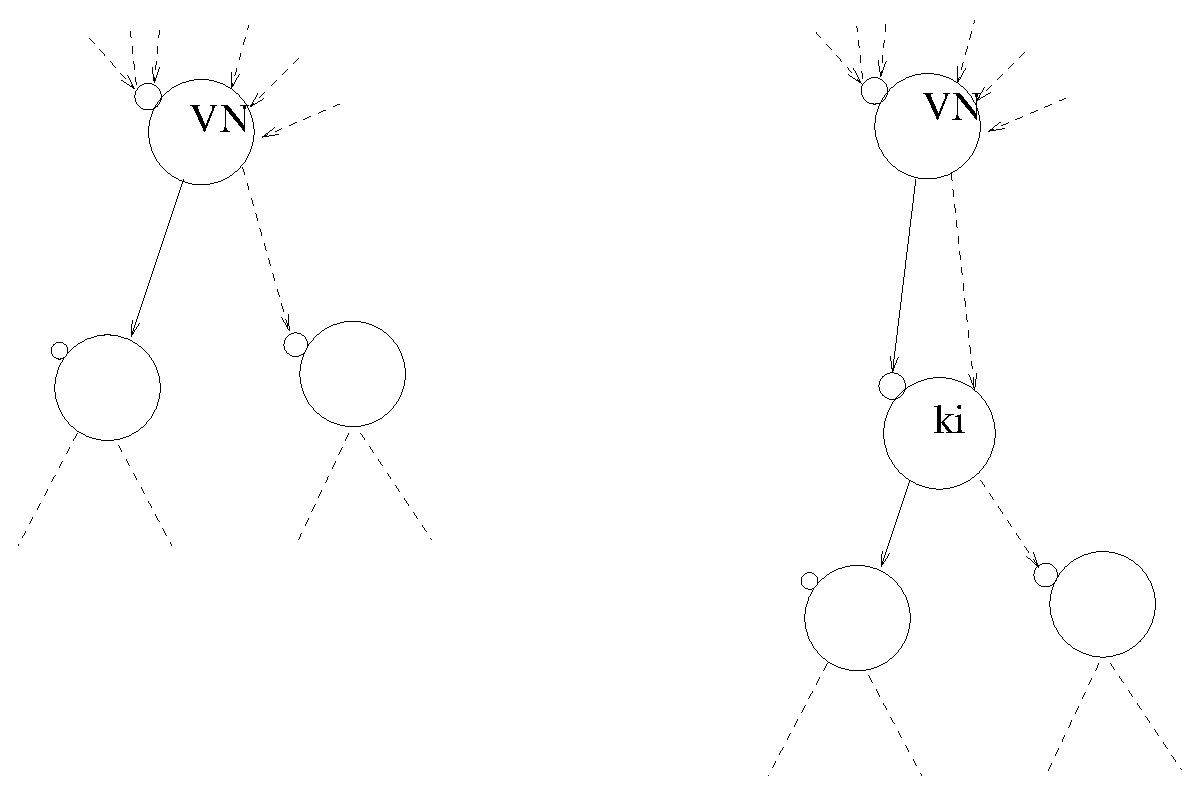
\includegraphics[scale=.5]{bubble_encrypt.eps}
%\caption{Digraph.}
%\label{fig:digraph}
%\end{figure*}

\begin{lemma}
Let $G_{k'}$ be the graph we get by eliminating key nodes in an encrypted BDD and making connections in accordance with the value of $k'$, and then replacing each bubbled node with its ``regular'' equivalent. Then $G$ is a BDD.
\end{lemma}

\begin{proof}
Assume not. Then $G$ must either contain nodes whose children are isomorphic (impossible, since there could not have been any in the original graph), or $G$ must contain subgraphs that are isomorphic. A pair of such subgraphs cannot be rooted by complement nodes, by definition; they also cannot be rooted by a pair of nodes ``originating" from different bubbled nodes (it would mean the original graph also had isomorphic subgraphs). No other possibilities remain, and thus no such pair of subgraphs can exist in the $G$. Hence, $G$ is also an ROBDD.
\end{proof}

\begin{lemma}
Each $G_{k'}$ is a distinct BDD.
\end{lemma}

\begin{theorem}
$s^{*}$ satisfies the necessary condition for secure synthesis of Proposition ??.
\end{theorem}

\begin{proof}
Let $f$ be the input description to $s*$, and denote by $c_k$ the output we get . Note that $c_k$ is a random variable. We need to show that for each $k\in K$, there exists a description $f_k$ that, when locked with $s^{*}$ using $k$ as a key, we get $c_k$; with the same probability for all $k$. This description is simply the Boolean circuit corresponding to $G_{k}$ for each $k$. Due to the fact that BDDs are canonical, we know we will obtain $G_{k}$ at the end of Step 1 of the procedure, if we provide such circuit as input to the locking procedure with $k$ as the locking key. All we need now is to show that the subset of nodes selected in the locking step is as likely to have been selected by $s^{*}$ as the corresponding set of nodes in the BDD of $f$, but since $s^{*}$ selects decision nodes for locking uniformly at random, this direcctly follows.
\end{proof}

this esse consists of inserting XOR gates at random plac
%In a bubbled BDD, rather than 
%Encryption in a bubbled BDD corresponds to inserting new bubbled nodes 

\subsection{Other Candidate Procedures}
Both notions of security defined above allow a much simpler construction for a secure procedure than our BDD idea. The construction is as follows: XOR $f$'s output with the output of a point function (whose password is the locking key), pass through an indistinguishability obfuscator, XOR the result with the output of a comparator that takes the input and key lines as arguments). The problem here of course is that the output corruptability for an incorrect netlist is very low. The BDD idea could have an advantage here.
